%
%    This program is free software; you can redistribute it and/or modify
%    it under the terms of the GNU General Public License as published by
%    the Free Software Foundation; either version 2 of the License, or
%    (at your option) any later version.
%
%    This program is distributed in the hope that it will be useful,
%    but WITHOUT ANY WARRANTY; without even the implied warranty of
%    MERCHANTABILITY or FITNESS FOR A PARTICULAR PURPOSE.  See the
%    GNU General Public License for more details.
%
%    You should have received a copy of the GNU General Public License
%    along with this program; if not, write to the Free Software
%    Foundation, Inc., 675 Mass Ave, Cambridge, MA 02139, USA.
%

% Version: $Revision$

%%%%%%%%%%%%%%%%
% Introduction %
%%%%%%%%%%%%%%%%

\section{Introduction}

The KnowledgeFlow provides an alternative to the Explorer as a
graphical front end to WEKA's core algorithms. The KnowledgeFlow is a
work in progress so some of the functionality from the Explorer is not
yet available. On the other hand, there are things that can be done in
the KnowledgeFlow but not in the Explorer.

\begin{center}
  \includegraphics[angle=270,width=10cm]{images/knowledgeflow/knowledgeflow.eps}
\end{center}

The KnowledgeFlow presents a \textit{data-flow} inspired interface to
WEKA. The user can select WEKA components from a tool bar, place them
on a layout canvas and connect them together in order to form a
\textit{knowledge flow} for processing and analyzing data. At present, all of
WEKA's classifiers, filters, clusterers, loaders and savers are
available in the KnowledgeFlow along with some extra tools.

The KnowledgeFlow can handle data either incrementally or in batches
(the Explorer handles batch data only). Of course learning from data
incrementally requires a classifier that can be updated on an instance
by instance basis. Currently in WEKA there are ten classifiers that
can handle data incrementally:
\begin{tight_itemize}
	\item AODE
	\item IB1
	\item IBk
	\item KStar
	\item NaiveBayesMultinomialUpdateable
	\item NaiveBayesUpdateable
	\item NNge
	\item Winnow
\end{tight_itemize}

\noindent And two of them are meta classifiers:
\begin{tight_itemize}
	\item \textit{RacedIncrementalLogitBoost} - that can use of any regression base
learner to learn from discrete class data incrementally.
	\item \textit{LWL} - locally weighted learning.
\end{tight_itemize}

%%%%%%%%%%%%
% Features %
%%%%%%%%%%%%

\newpage
\section{Features}

The KnowledgeFlow offers the following features:
\begin{itemize}
	\item intuitive data flow style layout
	\item process data in batches or incrementally 
	\item process multiple batches or streams in parallel (each separate flow 
  	executes in its own thread)
	\item chain filters together
	\item view models produced by classifiers for each fold in a cross validation
	\item visualize performance of incremental classifiers during 
  	processing (scrolling plots of classification accuracy, RMS error, 
  	predictions etc.)
        \item plugin facility for allowing easy addition of new components
        to the KnowledgeFlow
\end{itemize}

\newpage
\section{Components}
Components available in the KnowledgeFlow:

\subsection{DataSources} All of WEKA's loaders are available.
\begin{center}
	\epsfig{file=images/knowledgeflow/components_datasources.eps,height=2cm}
\end{center}

\subsection{DataSinks} All of WEKA's savers are available.
\begin{center}
	\epsfig{file=images/knowledgeflow/components_datasinks.eps,height=2cm}
\end{center}

\subsection{Filters} All of WEKA's filters are available.
\begin{center}
	\epsfig{file=images/knowledgeflow/components_filters.eps,height=2cm}
\end{center}

\subsection{Classifiers} All of WEKA's classifiers are available.
\begin{center}
	\epsfig{file=images/knowledgeflow/components_classifiers.eps,height=2cm}
\end{center}

\subsection{Clusterers} All of WEKA's clusterers are available.
\begin{center}
	\epsfig{file=images/knowledgeflow/components_clusterers.eps,height=2cm}
\end{center}

\subsection{Evaluation}
\begin{center}
	\epsfig{file=images/knowledgeflow/components_evaluation.eps,height=2cm}
\end{center}

\begin{itemize}
	\item \textit{TrainingSetMaker} - make a data set into a training set.
	\item \textit{TestSetMaker} - make a data set into a test set.
	\item \textit{CrossValidationFoldMaker} - split any data set, training 
	set or test set into folds.
	\item \textit{TrainTestSplitMaker} - split any data set, training set 
	or test set into a training set and a test set.
	\item \textit{ClassAssigner} - assign a column to be the class for any 
	data set, training set or test set.
	\item \textit{ClassValuePicker} - choose a class value to be considered 
	as the ``positive'' class. This is useful when generating data for ROC style 
	curves (see \textit{ModelPerformanceChart} below and example \ref{exampleroc}).
	\item \textit{ClassifierPerformanceEvaluator} - evaluate the performance of 
	batch trained/tested classifiers.
	\item \textit{IncrementalClassifierEvaluator} - evaluate the performance of 
	incrementally trained classifiers.
	\item \textit{ClustererPerformanceEvaluator} - evaluate the performance of 
	batch trained/tested clusterers.
	\item \textit{PredictionAppender} - append classifier predictions to a test 
	set. For discrete class problems, can either append predicted class labels or
	probability distributions.
\end{itemize}

\newpage
\subsection{Visualization}
\begin{center}
	\epsfig{file=images/knowledgeflow/components_visualization.eps,height=2cm}
\end{center}

\begin{itemize}
	\item \textit{DataVisualizer} - component that can pop up a panel for 
	visualizing data in a single large 2D scatter plot.
	\item \textit{ScatterPlotMatrix} - component that can pop up a panel 
	containing a matrix of small scatter plots (clicking on a small plot 
	pops up a large scatter plot).
	\item \textit{AttributeSummarizer} - component that can pop up a panel 
	containing a matrix of histogram plots - one for each of the attributes 
	in the input data.
	\item \textit{ModelPerformanceChart} - component that can pop up a 
	panel for visualizing threshold (i.e. ROC style) curves.
	\item \textit{TextViewer} - component for showing textual data. Can show 
	data sets, classification performance statistics etc.
	\item \textit{GraphViewer} - component that can pop up a panel for 
	visualizing tree based models.
	\item \textit{StripChart} - component that can pop up a panel that displays 
	a scrolling plot of data (used for viewing the online performance of 
	incremental classifiers).
\end{itemize}

%%%%%%%%%%%%
% Examples %
%%%%%%%%%%%%

\newpage
\section{Examples}

%%%%%%%%%%%%%%%%%%%%%%%%%%%%%%%%
% Example: cross-validated J48 %
%%%%%%%%%%%%%%%%%%%%%%%%%%%%%%%%

\subsection{Cross-validated J48}
Setting up a flow to load an ARFF file (batch mode) and
perform a cross-validation using J48 (WEKA's C4.5 implementation).

\begin{center}
	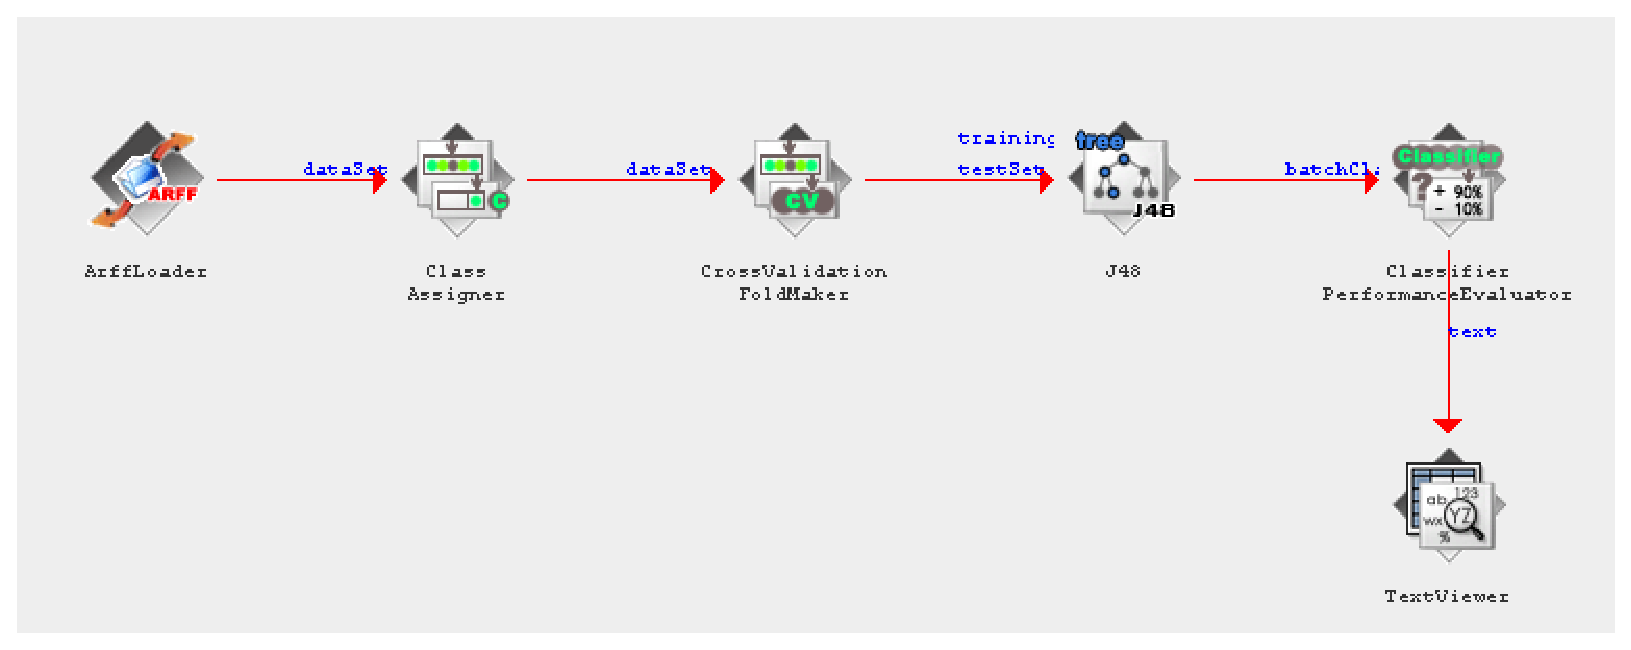
\epsfig{file=images/knowledgeflow/example_j48.eps,height=4.5cm}
\end{center}

\begin{itemize}
	\item Click on the DataSources tab and choose \textit{ArffLoader} from the
	toolbar (the mouse pointer will change to a \textit{cross hairs}).

	\item Next place the ArffLoader component on the layout area by clicking
	somewhere on the layout (a copy of the ArffLoader icon will appear on
	the layout area).

	\item Next specify an ARFF file to load by first right clicking the mouse
	over the ArffLoader icon on the layout. A pop-up menu will
	appear. Select \textit{Configure} under \textit{Edit} in the list from this menu and
	browse to the location of your ARFF file.

	\item Next click the \textit{Evaluation} tab at the top of the window and choose the
	\textit{ClassAssigner} (allows you to choose which column to be the class)
	component from the toolbar. Place this on the layout.

	\item Now connect the ArffLoader to the ClassAssigner: first right click
	over the ArffLoader and select the \textit{dataSet} under \textit{Connections} in
	the menu. A \textit{rubber band} line will appear. Move the mouse over the
	ClassAssigner component and left click - a red line labeled \textit{dataSet}
	will connect the two components.

	\item Next right click over the ClassAssigner and choose \textit{Configure} from
	the menu. This will pop up a window from which you can specify which
	column is the class in your data (last is the default).

	\item Next grab a \textit{CrossValidationFoldMaker} component from the Evaluation
	toolbar and place it on the layout. Connect the ClassAssigner to the
	CrossValidationFoldMaker by right clicking over \textit{ClassAssigner} and
	selecting \textit{dataSet} from under \textit{Connections} in the menu.

	\item Next click on the \textit{Classifiers} tab at the top of the window and
	scroll along the toolbar until you reach the \textit{J48} component in the
	\textit{trees} section. Place a J48 component on the layout.

	\item Connect the CrossValidationFoldMaker to J48 TWICE by first choosing
	\textit{trainingSet} and then \textit{testSet} from the pop-up menu for the
	CrossValidationFoldMaker.

	\item Next go back to the \textit{Evaluation} tab and place a
	\textit{ClassifierPerformanceEvaluator} component on the layout. Connect J48
	to this component by selecting the \textit{batchClassifier} entry from the
	pop-up menu for J48.

	\item Next go to the \textit{Visualization} toolbar and place a \textit{TextViewer}
	component on the layout. Connect the ClassifierPerformanceEvaluator to
	the TextViewer by selecting the \textit{text} entry from the pop-up menu for
	ClassifierPerformanceEvaluator.

	\item Now start the flow executing by selecting \textit{Start loading} from the
	pop-up menu for ArffLoader. Depending on how big the data set is and
	how long cross-validation takes you will see some animation from some
	of the icons in the layout (J48's tree will \textit{grow} in the icon and the
	ticks will animate on the ClassifierPerformanceEvaluator). You will
	also see some progress information in the \textit{Status} bar and \textit{Log} at
	the bottom of the window.
\end{itemize}

When finished you can view the results by choosing \textit{Show results} from
the pop-up menu for the \textit{TextViewer} component.

Other cool things to add to this flow: connect a \textit{TextViewer} and/or a
\textit{GraphViewer} to J48 in order to view the textual or graphical
representations of the trees produced for each fold of the cross
validation (this is something that is not possible in the Explorer).

%%%%%%%%%%%%%%%%%%%%%%%%%
% Example: multiple ROC %
%%%%%%%%%%%%%%%%%%%%%%%%%

\newpage
\subsection{Plotting multiple ROC curves}
\label{exampleroc}
The KnowledgeFlow can draw multiple ROC curves in the same plot window, something that the 
Explorer cannot do. In this example we use \textit{J48} and \textit{RandomForest}
as classifiers. This example can be found on the \textit{WekaWiki} as well \cite{multipleroc}.

\begin{center}
	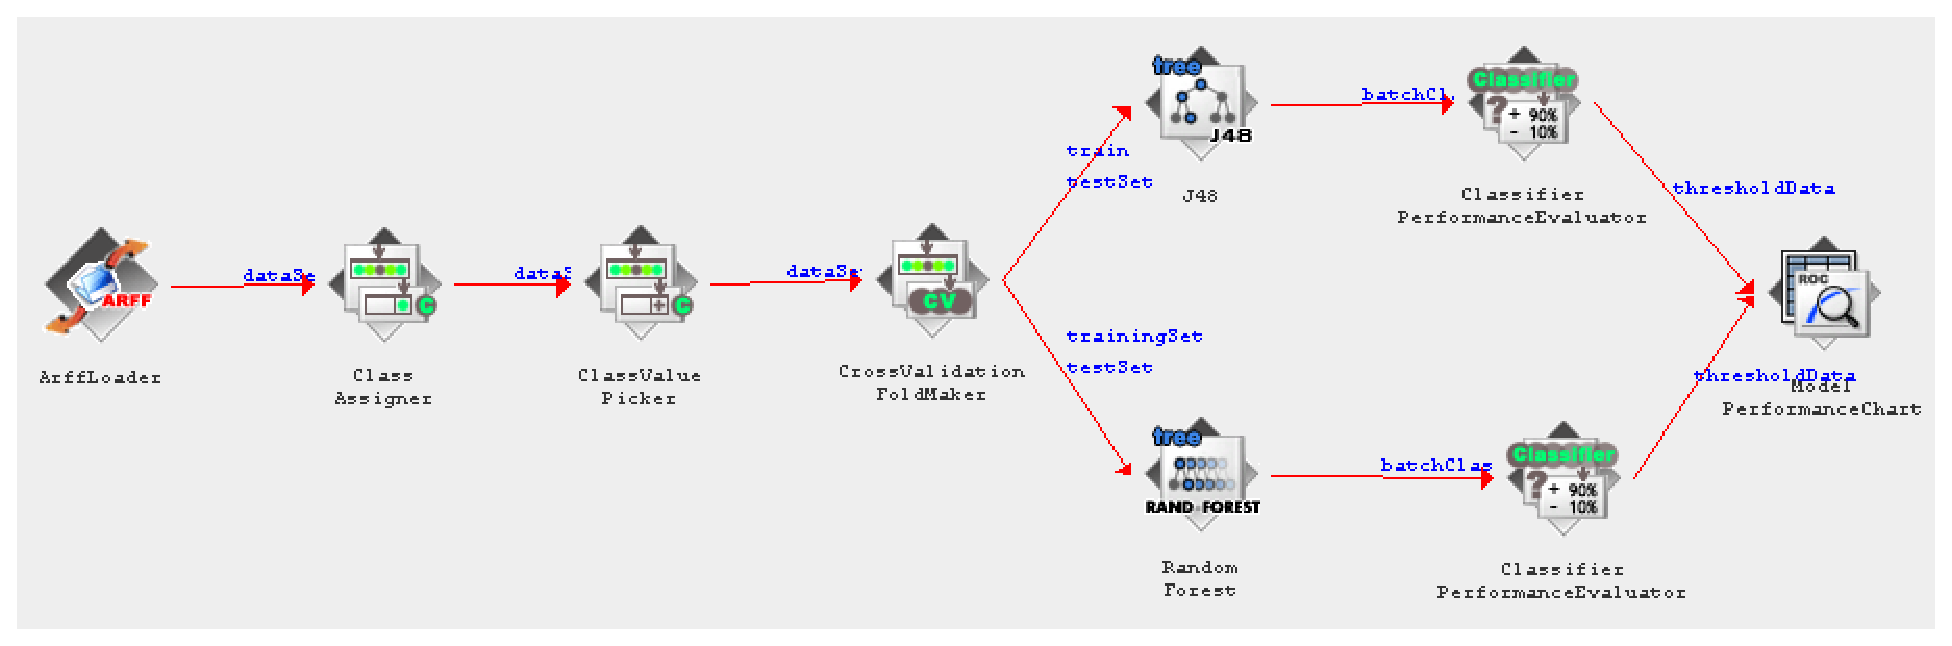
\epsfig{file=images/knowledgeflow/example_multiple_roc.eps,height=4cm}
\end{center}

\begin{itemize}
	\item Click on the DataSources tab and choose \textit{ArffLoader} from the
	toolbar (the mouse pointer will change to a \textit{cross hairs}).

	\item Next place the ArffLoader component on the layout area by clicking
	somewhere on the layout (a copy of the ArffLoader icon will appear on
	the layout area).

	\item Next specify an ARFF file to load by first right clicking the mouse
	over the ArffLoader icon on the layout. A pop-up menu will
	appear. Select \textit{Configure} under \textit{Edit} in the list from this menu and
	browse to the location of your ARFF file.

	\item Next click the \textit{Evaluation} tab at the top of the window and choose the
	\textit{ClassAssigner} (allows you to choose which column to be the class)
	component from the toolbar. Place this on the layout.

	\item Now connect the ArffLoader to the ClassAssigner: first right click
	over the ArffLoader and select the \textit{dataSet} under \textit{Connections} in
	the menu. A \textit{rubber band} line will appear. Move the mouse over the
	ClassAssigner component and left click - a red line labeled \textit{dataSet}
	will connect the two components.

	\item Next right click over the ClassAssigner and choose \textit{Configure} from
	the menu. This will pop up a window from which you can specify which
	column is the class in your data (last is the default).

	\item Next choose the \textit{ClassValuePicker} (allows you to choose which class 
	label to be evaluated in the ROC) component from the toolbar. Place this on the layout
	and right click over \textit{ClassAssigner} and select \textit{dataSet} from under
	\textit{Connections} in the menu and connect it with the \textit{ClassValuePicker}.

	\item Next grab a \textit{CrossValidationFoldMaker} component from the Evaluation
	toolbar and place it on the layout. Connect the ClassAssigner to the
	CrossValidationFoldMaker by right clicking over \textit{ClassAssigner} and
	selecting \textit{dataSet} from under \textit{Connections} in the menu.

	\item Next click on the \textit{Classifiers} tab at the top of the window and
	scroll along the toolbar until you reach the \textit{J48} component in the
	\textit{trees} section. Place a J48 component on the layout.

	\item Connect the CrossValidationFoldMaker to J48 TWICE by first choosing
	\textit{trainingSet} and then \textit{testSet} from the pop-up menu for the
	CrossValidationFoldMaker.

	\item Repeat these two steps with the RandomForest classifier.

	\item Next go back to the \textit{Evaluation} tab and place a
	\textit{ClassifierPerformanceEvaluator} component on the layout. Connect J48
	to this component by selecting the \textit{batchClassifier} entry from the
	pop-up menu for J48. Add another \textit{ClassifierPerformanceEvaluator} for
	RandomForest and connect them via \textit{batchClassifier} as well.

	\item Next go to the \textit{Visualization} toolbar and place a 
	\textit{ModelPerformanceChart} component on the layout. Connect both 
	ClassifierPerformanceEvaluators to the ModelPerformanceChart by selecting 
	the \textit{thresholdData} entry from the pop-up menu for ClassifierPerformanceEvaluator.

	\item Now start the flow executing by selecting \textit{Start loading} from the
	pop-up menu for ArffLoader. Depending on how big the data set is and
	how long cross validation takes you will see some animation from some
	of the icons in the layout. You will also see some progress information in the 
	\textit{Status} bar and \textit{Log} at the bottom of the window.
	
	\item Select \textit{Show plot} from the popup-menu of the 
	\textit{ModelPerformanceChart} under the \textit{Actions} section.
\end{itemize}

Here are the two ROC curves generated from the UCI dataset \textit{credit-g}, 
evaluated on the class label \textit{good}:

\begin{center}
	\epsfig{file=images/knowledgeflow/example_multiple_roc_output.eps,height=8.5cm}
\end{center}

%%%%%%%%%%%%%%%%%%%%%%%%%%%%%%%%%%%%%%%%%%%
% Example: processing data incrementally  %
%%%%%%%%%%%%%%%%%%%%%%%%%%%%%%%%%%%%%%%%%%%

\newpage
\subsection{Processing data incrementally}

Some classifiers, clusterers and filters in Weka can handle data incrementally
in a streaming fashion. Here is an example of training and testing \textit{naive Bayes}
incrementally. The results are sent to a \textit{TextViewer} and predictions are plotted
by a \textit{StripChart} component.

\begin{center}
  \includegraphics[angle=270,width=13cm]{images/knowledgeflow/IncrementalFlow.eps}
\end{center}

\begin{itemize}
        \item Click on the DataSources tab and choose \textit{ArffLoader} from the
	toolbar (the mouse pointer will change to a \textit{cross hairs}).

	\item Next place the ArffLoader component on the layout area by clicking
	somewhere on the layout (a copy of the ArffLoader icon will appear on
	the layout area).

	\item Next specify an ARFF file to load by first right clicking the mouse
	over the ArffLoader icon on the layout. A pop-up menu will
	appear. Select \textit{Configure} under \textit{Edit} in the list from this menu and
	browse to the location of your ARFF file.

	\item Next click the \textit{Evaluation} tab at the top of the window and choose the
	\textit{ClassAssigner} (allows you to choose which column to be the class)
	component from the toolbar. Place this on the layout.

	\item Now connect the ArffLoader to the ClassAssigner: first right click
	over the ArffLoader and select the \textit{dataSet} under \textit{Connections} in
	the menu. A \textit{rubber band} line will appear. Move the mouse over the
	ClassAssigner component and left click - a red line labeled \textit{dataSet}
	will connect the two components.

	\item Next right click over the \textit{ClassAssigner} and choose \textit{Configure} from
	the menu. This will pop up a window from which you can specify which
	column is the class in your data (last is the default).

        \item Now grab a \textit{NaiveBayesUpdateable} component from the \textit{bayes}
        section of the \textit{Classifiers} panel and place it on the layout.

        \item Next connect the \textit{ClassAssigner} to \textit{NaiveBayesUpdateable}
        using a \textit{instance} connection.

        \item Next place an \textit{IncrementalClassiferEvaluator} from the \textit{Evaluation}
        panel onto the layout and connect \textit{NaiveBayesUpdateable} to it using a
        \textit{incrementalClassifier} connection.

        \item Next place a \textit{TextViewer} component from the \textit{Visualization}
        panel on the Layout. Connect the \textit{IncrementalClassifierEvaluator} to
        it using a \textit{text} connection.

        \item Next place a \textit{StripChart} component from the \textit{Visualization}
        panel on the layout and connect \textit{IncrementalClassifierEvaluator} to it
        using a \textit{chart} connection.

        \item Display the \textit{StripChart's} chart by right-clicking over it and choosing
        \textit{Show chart} from the pop-up menu. Note: the \textit{StripChart} can be configured
        with options that control how often data points and labels are displayed.

        \item Finally, start the flow by right-clicking over the \textit{ArffLoader} and
        selecting \textit{Start loading} from the pop-up menu.        
\end{itemize}

\begin{center}
  \includegraphics[angle=270,width=12cm]{images/knowledgeflow/IncrementalChart.eps}
\end{center}

Note that, in this example, a prediction is obtained from naive Bayes
for each incoming instance {\bf before} the classifier is trained
(updated) with the instance. If you have a pre-trained classifier, you
can specify that the classifier {\bf not} be updated on incoming
instances by unselecting the check box in the configuration dialog for
the classifier. If the pre-trained classifier is a {\bf batch}
classifier (i.e. it is not capable of incremental training) then you
will only be able to test it in an incremental fashion.

\begin{center}
  \includegraphics[angle=270,width=12cm]{images/knowledgeflow/IncrementalClassifierConfig.eps}
\end{center}

\newpage
\section{Plugin Facility}

The KnowledgeFlow offers the ability to easily add new components via
a plugin mechanism. Plugins are installed in a directory called
\verb=.knowledgeFlow/plugins= in the user's home directory. If this
directory does not exist you must create it in order to install
plugins. Plugins are installed in subdirectories of the
\verb=.knowledgeFlow/plugins= directory. More than one plugin
component may reside in the same subdirectory. Each subdirectory
should contain jar file(s) that contain and support the plugin
components. The KnowledgeFlow will dynamically load jar files and add
them to the classpath. In order to tell the KnowledgeFlow which
classes in the jar files to instantiate as components, a second file
called \verb=Beans.props= needs to be created and placed into each
plugin subdirectory. This file contains a list of fully qualified
class names to be instantiated. Successfully instantiated components
will appear in a ``Plugins'' tab in the KnowledgeFlow user
interface.Below is an example plugin directory listing, the listing of
the contents of the jar file and the contents of the associated
Beans.props file:

\begin{verbatim}
cygnus:~ mhall$ ls -l $HOME/.knowledgeFlow/plugins/kettle/
total 24
-rw-r--r--   1 mhall  mhall   117 20 Feb 10:56 Beans.props
-rw-r--r--   1 mhall  mhall  8047 20 Feb 14:01 kettleKF.jar

cygnus:~ mhall$ jar tvf /Users/mhall/.knowledgeFlow/plugins/kettle/kettleKF.jar 
     0 Wed Feb 20 14:01:34 NZDT 2008 META-INF/
    70 Wed Feb 20 14:01:34 NZDT 2008 META-INF/MANIFEST.MF
     0 Tue Feb 19 14:59:08 NZDT 2008 weka/
     0 Tue Feb 19 14:59:08 NZDT 2008 weka/gui/
     0 Wed Feb 20 13:55:52 NZDT 2008 weka/gui/beans/
     0 Wed Feb 20 13:56:36 NZDT 2008 weka/gui/beans/icons/
  2812 Wed Feb 20 14:01:20 NZDT 2008 weka/gui/beans/icons/KettleInput.gif
  2812 Wed Feb 20 14:01:18 NZDT 2008 weka/gui/beans/icons/KettleInput_animated.gif
  1839 Wed Feb 20 13:59:08 NZDT 2008 weka/gui/beans/KettleInput.class
   174 Tue Feb 19 15:27:24 NZDT 2008 weka/gui/beans/KettleInputBeanInfo.class

cygnus:~ mhall$ more /Users/mhall/.knowledgeFlow/plugins/kettle/Beans.props 
# Specifies the tools to go into the Plugins toolbar
weka.gui.beans.KnowledgeFlow.Plugins=weka.gui.beans.KettleInput
\end{verbatim}
